\subsection{Числа Каталана}

\subsubsection*{Правильная скобочная последовательность (ПСП)}

\begin{defn}
    Язык строк над $\sum = \{ (, ) \}$

    Определение по индукции:

    \begin{itemize}
        \item пустая строка $\eps$ --- ПСП;
        \item если $w$ --- ПСП, то $(w)$ --- ПСП;
        \item если $w, u$ --- ПСП, то $w u$ --- ПСП.
    \end{itemize}

    Множество ПСП называется языком Дика:\\
    $\eps,~(),~(()),~()(),~((())),~()(()),~((()())),~\dots$
\end{defn}

Сколько существует ПСП с $n$ парами скобок (= сколько слов длины $2n$ в языке Дика)?

Это задается последовательностью чисел Каталана $C_n$.

\subsubsection*{Реккурентная формула для чисел Каталана}

\begin{theorem} (реккурентная формула)
    \[ C_0 = 1;~C_{n} = \sum_{k = 0}^{n - 1} C_i C_{n - 1 - k} \]
\end{theorem}

\begin{proof}
    Пусть $w$ --- произвольная ПСП длины $2n$.

    Она начинается с открывающейся скобки. Найдем парную ей закрывающуюся скобку и представим последовательность $w$ в виде: $w = (u)v$, где $u$ и $v$ ПСП.

    Если длина $u$ равна $2k$, то $u$ можно составить $D_k$ способами. 

    Тогда длина $v$ равна $2(n - k - 1)$ и $v$ можно составить $D_{n - k - 1}$ способами.

    Комбинация любого способа составить $u$ с любым спосбом составить $v$ даст новую последовательность $w$.

    Суммируя по $k$ от $0$ до $n - 1$ получаем рекуррентую формулу.
\end{proof}

\subsubsection*{Числа Каталана через монотонные пути}

ПСП длины $2n$ постаим в соответствие путь в квадрате $[0,n] \times [0,n]$ из точки $(0, 0)$ в точку $(n, n)$.

Открывающей скобке сопоставим горизонтальный отрезок длины $1$, а закрывающей --- вертикальный отрезок длины $1$.

\begin{center}
    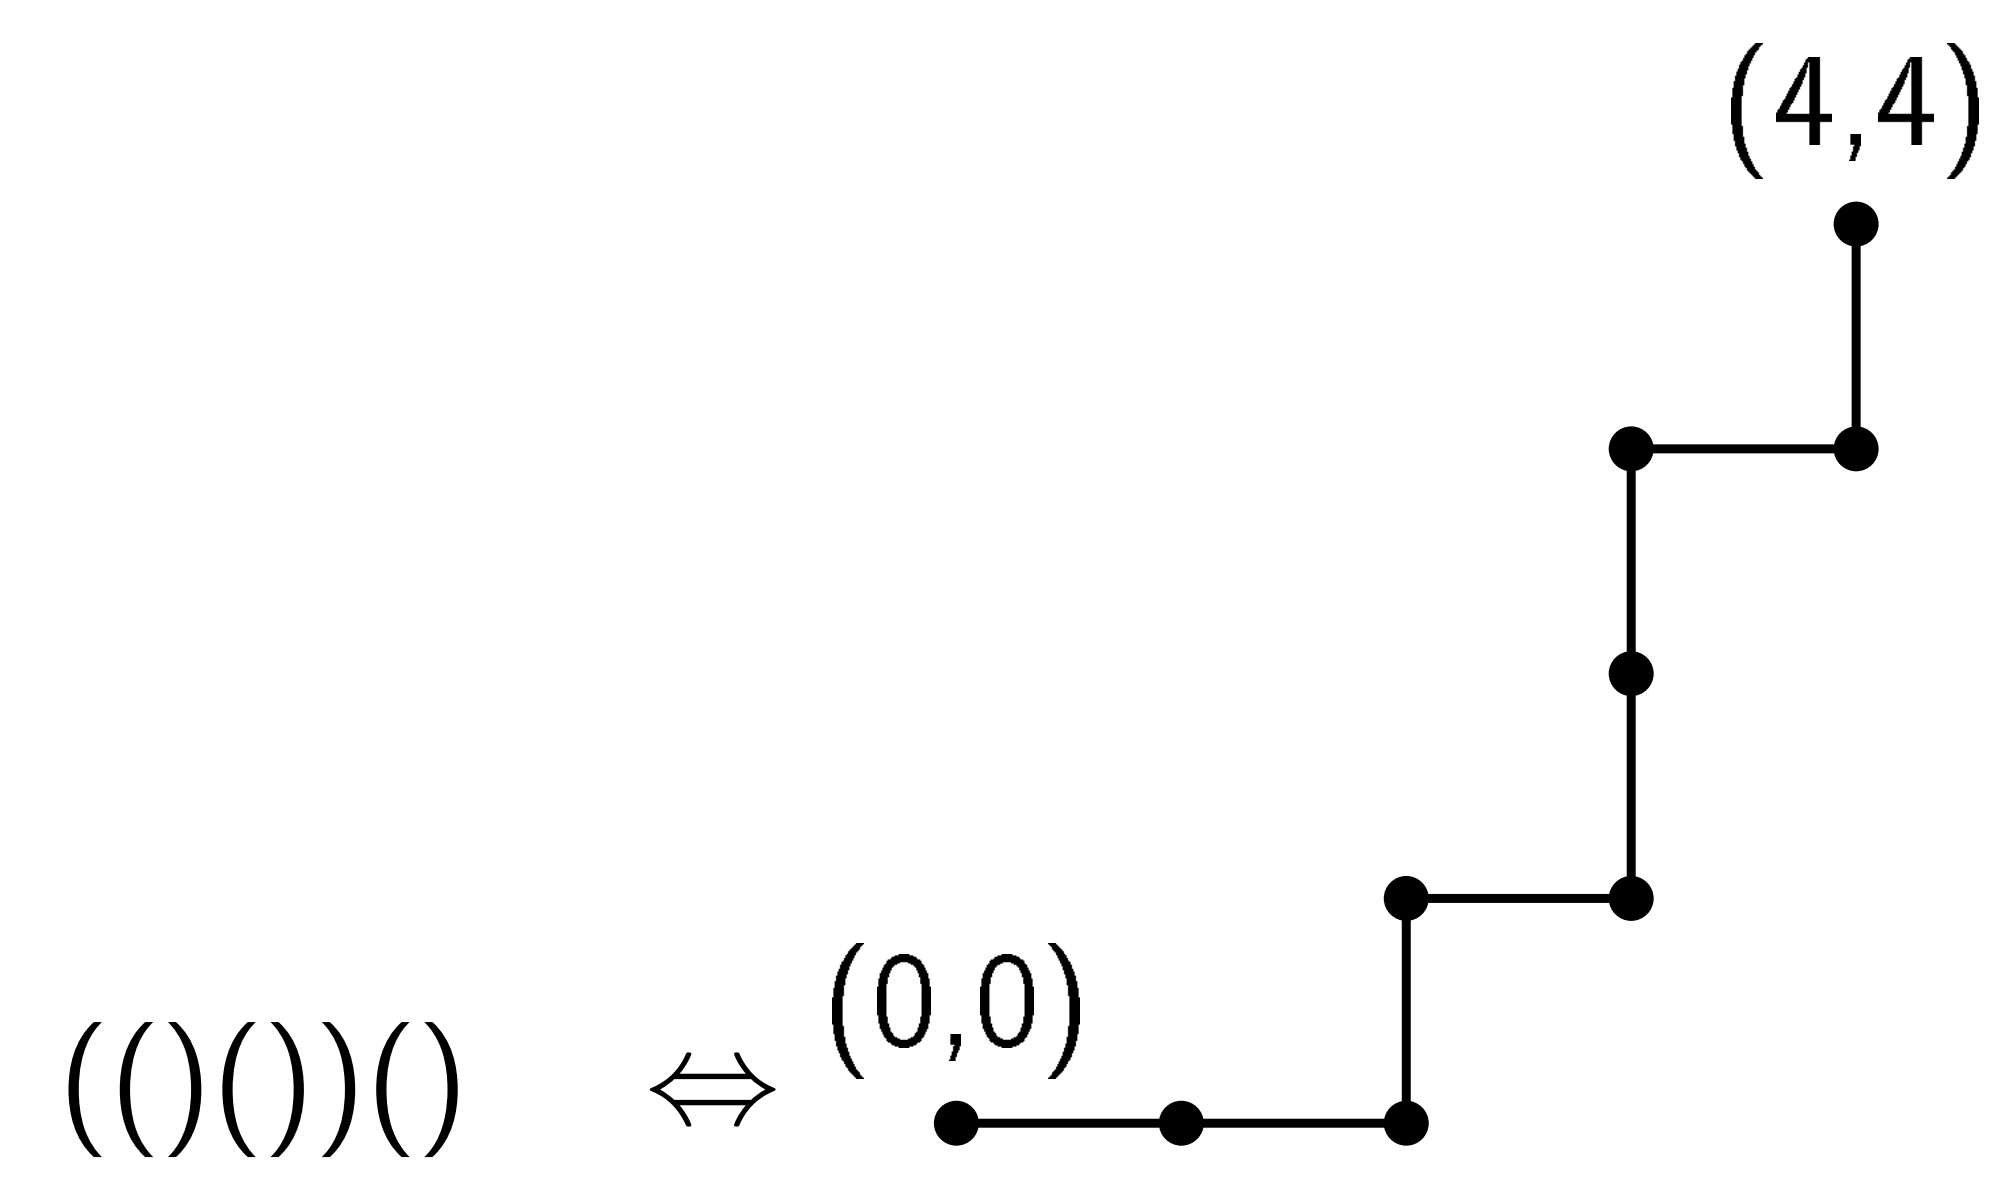
\includegraphics[width=0.5\textwidth]{par16path.png}
\end{center}
Если путь сопоставлен ПСП, то ни одна его точка не может лежать выше главной диагонали квадрата (<<правильный путь>>). Обратно, такому пути сопоставляется ПСП.

\subsubsection*{Аналитическая формула для чисел Каталана}

\begin{theorem}
    \[ C_n = \frac{1}{n + 1} C_{2n}^n \]
\end{theorem}

\begin{proof}

    Сместим правильный путь на $1$ клетку вниз. Теперь правильный путь идет из $(0, -1)$ в $(n, n - 1)$ и не имеет общих точек с прямой $y = x$.

    Число правильных путей = общее число путей - число неправильных.

    Общее число путей из $(0, -1)$ в $(n, n - 1)$ --- число способов выбрать $n$ вертикальных сегментов (и $n$ горизонтальных) из общего числа $2n$, то есть $C_{2n}^n$.

    Рассмотрим неправильный путь и его первую точку на прямой $y = x$ (точка $A$). Отрезок пути от $(0, -1)$ до $A$ заменим симметричным относительно прямой $y = x$. Получим путь длины $2n$ из $(-1, 0)$ в $(n, n - 1)$.

    \begin{center}
        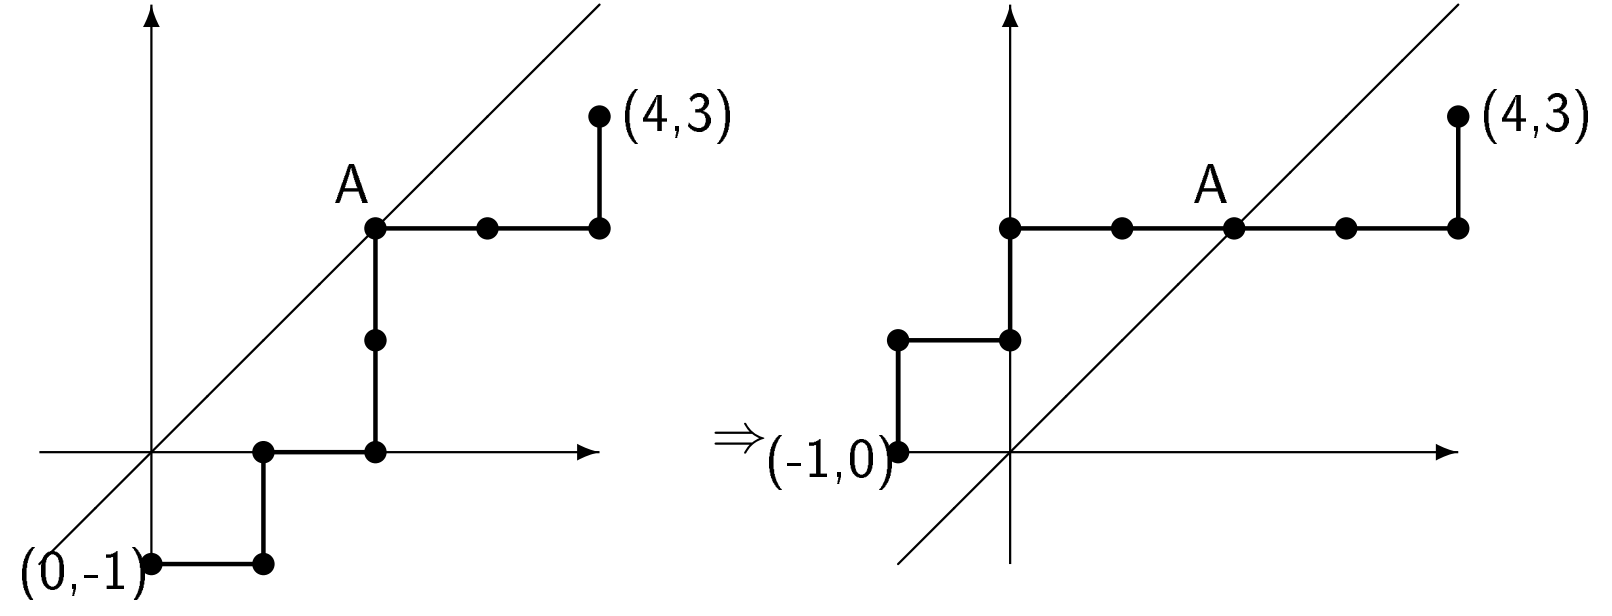
\includegraphics[width=0.5\textwidth]{par16proof.png}
    \end{center}

    Обратно, пусть дан путь длины $2n$ из $(-1, 0)$ в $(n, n - 1)$ и пусть $A$ --- первая точка этого пути на прямой $y = x$. 

    Заменив участок пути от $(-1, 0)$ до $A$ на симметричный относительно прямой $y = x$, получим неправильный путь из $(0, -1)$ в $(n, n - 1)$.

    Следовательно, неправильных путей из $(0, -1)$ в $(n, n - 1)$ столько же, сколько путей из точки из $(-1, 0)$ в $(n, n - 1)$.

    Путь из $(-1, 0)$ в $(n, n - 1)$ содержит $n + 1$ горизонтальных и $n - 1$ вертикальных участков. Поэтому количество таких путей равно $C_{2n}^{n - 1}$.

    Значит, количество правильных путей (то есть число Каталана $C_n$) равно \[ C_n = C_{2n}^n - C_{2n}^{n - 1} = \frac{2n!}{n!n!} - \frac{2n!}{(n - 1)!(n + 1)!} = \frac{2n!}{n!(n + 1)!} = \frac{1}{(n + 1)} C_{2n}^n. \]

\end{proof}

\subsubsection*{Асимтотика чисел Каталана}

\begin{theorem}
    
    \[ C_n = (1 + o(1)) \frac{4^n}{n^{\frac{3}{2}} \sqrt{\pi}} \]

\end{theorem}

\begin{proof}
    
    Используем формулу Стирлинга:

    \[ n! = (1 + o(1)) \sqrt{2 \pi n} \left( \frac{n}{e} \right)^n \]

    Оценим биномиальный коэффицент:

    \[ C_{2n}^n = \frac{2n!}{(n!)^2} = \frac{ (1 + o(1)) \sqrt{2 \pi 2 n} \left( \frac{2n}{e} \right)^{2n}}{ (1 + o(1)) 2 \pi n \left( \frac{n}{e} \right)^{2n}} = (1 + o(1)) \frac{4^n}{\sqrt{\pi n}} \]

    Далее, число Каталана

    \[ \frac{1}{n + 1} C_{2n}^n = (1 + o(1)) \frac{1}{n + 1} \frac{4^n}{\sqrt{\pi n}} = (1 + o(1)) \frac{4^n}{n^{\frac{3}{2}} \sqrt{\pi}} \]

\end{proof}

\subsubsection*{Другие представления чисел Каталана}

\begin{itemize}
    \item число разбиений выпуклого $(n + 2)$-угольника на треугольники непересекающимися диагоналями.
    
    \item число способов соединения $2n$ точек на окружности $n$ непересекающимися хордами
    
    \item число способов заполнить $n$-лесенку $n$ прямоугольниками
    
    \item число таблиц Юнга размером $2 \times n$. Таблица Юнга --- прямоугольник, заполненный последовательными числами так, чтобы они возрастали во всех строках и столбцах:
    
    $1 \quad 2 \quad 4$\\
    $3 \quad 5 \quad 6$\\

    \item число плоских корневых деревьев с $n + 1$ вершинами

    \item число неизоморфных корневых деревьев с $n + 1$ вершинами
    
    \item число параллеломино (пар путей на клетчатой бумаге с началом $(0, 0)$ и концом в одной и той же точке, идущих только вверх и вправо и не имеющихся общих точек, кроме начала и конца) периметра $2n + 2$
    
    \item число последовательностей натуральных чисел $1, a_1, \ldots, a_n, 1$ в которых каждый член является делителем суммы двух соседей:
    
    $1~4~3~2~1, 1~3~5~2~1, 1~3~2~3~1, 1~2~5~3~1, 1~2~3~4~1$

    \item число наборов из $n$ целых чисел от $0$ до $n$, сумма которых делится на $(n + 1)$
    
    $0~0~0, 0~1~3, 0~2~2, 1~1~2, 2~3~3$

    \item число способов разделить скобками $(n + 1)$ множитель
\end{itemize}